\documentclass[13pt,oneside]{book}
\usepackage[utf8]{inputenc}
\usepackage{url}
\usepackage{listings}
\usepackage{graphicx}

\usepackage{geometry}
\geometry{a4paper, left=20mm, right=20mm, top=20mm, bottom=20mm}
\usepackage[margin=1.2in]{geometry}
\usepackage[toc,page]{appendix}
\usepackage{graphicx}
\usepackage{natbib}
\usepackage{lipsum}
\usepackage{caption}

\begin{document}

\captionsetup[figure]{margin=1.5cm,font=small,labelfont={bf},name={Figure},labelsep=colon,textfont={it}}
\captionsetup[table]{margin=1.5cm,font=small,labelfont={bf},name={Table},labelsep=colon,textfont={it}}
\setlipsumdefault{1}

\begin{titlepage}
\begin{center}
{\LARGE College Of Engineering Trivandrum}\\[3cm]
\linespread{1.2}\huge {\bfseries System Software Lab}\\[3cm]
\linespread{1}

\includegraphics[width=5cm]{img/emblem.jpeg}\\[3cm]
{\Large GOKUL K\\ S5  CSE \\ Roll No:21\\ TVE18CS021 }\\[1cm]


\textit{ }\\[2cm]
Department of Computer Science\\[0.2cm]
\today
\end{center}

\end{titlepage}

\newpage

\begin{frame}{}
    \centering
    \hspace*{-0.5cm}
    $\vcenter{\hbox{
\includegraphics[width=1.5cm]{img/emblem.jpeg}}}$
    $\vcenter{\resizebox{0.95\textwidth}{!}{
        \begin{tabular}{c}
             CS331 - System Software Lab $\cdot$ 2020 $\cdot$   \\
             \hline 
        \end{tabular}
    }}$
\end{frame}
\section*{Cycle 1}
\section*{Expt 4}
\begin{center}
    \Large{Banker\'s Algorithm}
\end{center}FCFS
\section*{Aim}
\large
Implement the banker’s algorithm for deadlock avoidance.

\section*{Algorithm}
    \begin{verbatim}
		Implement the banker’s algorithm for deadlock avoidance.
    \end{verbatim}  
    \subsection*{LRU}
    \begin{verbatim}
	1 If Requesti = Needi , go to step 2. Otherwise , raise an error
	condition ,
	2 since the process has exceeded its maximum claim .
	3 If Requesti = Available , go to step 3. Otherwise , Pi must wait ,
	since the
	4 resources are not available .
	5 Have the system pretend to have allocated the requested resources
	to
	6 process , Pi by modify the state as follows :
	7 Available = Available - Requesti ;
	8 Allocationi = Allocationi + Requesti ;
	9 Needi = Needi - Requesti ;
	\end{verbatim}

\section*{Source Code}
\small

\begin{lstlisting}[language=C]
#include <string.h>
#include <stdio.h>
#include <stdlib.h>

#define PROC_NO 5
#define RES_NO 3

struct Process
{
	char *proc_name;
	int *current_alloc;
	int *max_req;
	int finished;
};

int tot_res[3] = {10, 5, 7};

struct Process *create_process()
{
	/* Reads process details */

	struct Process *process = malloc(sizeof(struct Process));
	int *current_alloc = malloc(3 * sizeof(int));
	int *max_req = malloc(3 * sizeof(int));
	process->proc_name = malloc(20 * sizeof(char));

	printf("Enter process name: ");
	scanf("%[^\n]%*c", process->proc_name);

	printf("Enter current allocations of A, B and C: ");
	scanf("%d %d %d%*c", current_alloc, (current_alloc + 1), (current_alloc + 2));

	printf("Enter maximum requirements: ");
	scanf("%d %d %d%*c", max_req, max_req + 1, max_req + 2);

	process->current_alloc = current_alloc;
	process->max_req = max_req;
	process->finished = 0;

	return process;
}

struct Process **get_processes()
{
	/* Returns the process table */

	int i;
	struct Process **proc_table = malloc(PROC_NO * sizeof(struct Process));
	for(i = 0; i < PROC_NO; i++)
		proc_table[i] = create_process();
	
	return proc_table;
}

int *get_requests(struct Process **proc_table)
{
	/* Reads resource request from a process */

	int i, j, req;
	int *req_table = malloc(PROC_NO * RES_NO * sizeof(int));

	for(i = 0; i < PROC_NO; i++)
	{
		printf("Request for %s: ", proc_table[i]->proc_name);
		for(j = 0; j < RES_NO; j++)
		{
			scanf("%d", &req);
			*(req_table + i*RES_NO + j) = req;
		}
			
		printf("\n");
	}

	return req_table;
}



int *calculate_available(struct Process **proc_table) 
{
	/* Calculate the remaining resources */

	int *avialable = malloc(3 * sizeof(int)), i, j, sum;

	for(i = 0; i < RES_NO; i++)
	{
		sum = 0;
		for(j = 0; j < PROC_NO; j++)
			sum += proc_table[j]->current_alloc[i];

		avialable[i] = tot_res[i] - sum;
	}

	return avialable;
} 

int is_safe(struct Process **proc_table, int *available, char *seq)
{
	/* Check if the system is safe and to store the sequence of 
	allocation */

	int i = 0, j, repeat = 0, is_finished = 1, finished_count = 0, need;

	for(i = 0; i < PROC_NO; i++)
	{
		if(!proc_table[i]->finished)
		{
			is_finished = 1;
			for(j = 0; j < RES_NO; j++)
			{
				need = proc_table[i]->max_req[j] - proc_table[i]->current_alloc[j];
				is_finished = is_finished && (available[j] >= need);
			}

			if(is_finished)
			{
				repeat = 1;
				for(j = 0; j < RES_NO; j++)
					available[j] += proc_table[i]->current_alloc[j];
				proc_table[i]->finished = 1;
				strcat(seq, proc_table[i]->proc_name);
				finished_count++;
				strcat(seq, (finished_count != PROC_NO) ? " -> " : "");
			}
		}

		if(i == PROC_NO-1 && repeat)
		{
			i = -1;
			repeat = 0;
		}
	}

	return finished_count == PROC_NO;
}


int main()
{
	struct Process** proc_table = get_processes();
	int i = 0, *avialable;

	char *s = malloc(30 * sizeof(char));
	
	avialable = calculate_available(proc_table);

	if(is_safe(proc_table, avialable, s))
		printf("The system is safe\n%s\n", s);
	else
		printf("The system is unsafe\n");

	free(proc_table);
	free(avialable);
	free(s);
	}
    \end{lstlisting}
    \section*{Output}
    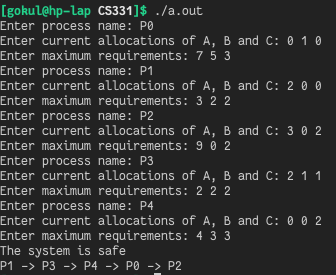
\includegraphics[]{img/p4.png}
    
\Large
\section*{Result}
\large
The banker's algorithm were implemented and its output verified
\end{document}